In this strategy, mesh refinement is applied around dominant flow features of interest. 
In the surging airfoil case, LEV and TEV are the dominant flow features. 
Using vortex tracking, a path of the dominant vortices is estimated using an initial mesh (M0\_nz25 in this case). 
Based on this path, a refinement zone is added around the path of the LEV as well as the TEV. 
In this feature-based refinement, VMS-based estimated error is used to set the mesh size. 
In addition, estimated error is also used to refine the mesh around the airfoil in a similar fashion as the error-based zonal refinement discussed earlier. 
This is done to accurately resolve the flow near the airfoil, including the boundary layer region that plays a direct role in the formation of these dominant vortical structures/features.

Also note that the boundary layer mesh is refined by a factor of 2 in the streamwise direction, and the number of layers in the spanwise direction are doubled as compared to M0\_nz25.  
Vortex tracking discussed in Section \ref{sec:LEV} is used to estimate the path of the LEV and TEV. 
The mesh around the path of these vortical features is refined by a factor of 4, to accurately resolve the core of these vortices over its path. 
The mesh is referred to as Mfa1\_nz50 and it contains 3,454,450 elements.
This mesh is shown in Figure \ref{fig:FB_mesh} and the estimated error is shown in Figure \ref{fig:FB_error_plot}.

Error values along the LEV path are reduced as compared to Msa1\_nz50 and Mza1\_nz50, since a factor of 4 refinement is used instead of a factor of 2 to accurately resolve the LEV core along its path.
Error values are similar to Mza1\_nz50 closer to the airfoil surface and in the wake, since the mesh resolution in this region is similar.
Error values are lower as compared to Msa1\_nz50 closer to the airfoil surface and in the wake, since a uniform mesh size is maintained, as opposed to Msa1\_nz50, where the mesh size is patchy.

%Even though the mesh resolution in the LEV region is similar to Mza2\_nz5, higher error is observed as compared to Mz\_a2, since the mesh resolution over the airfoil surface is coarser for Mf\_a1 as compared to Mz\_a2.

\begin{figure}[H]
\centering

\begin{subfigure}[b]{0.475\textwidth}
\centering
\includegraphics[width=1\textwidth]{figures/adapt_strat/FB_mesh.png}
\caption{Mfa1\_nz50 mesh}
\label{fig:FB_mesh}
\end{subfigure}
\begin{subfigure}[b]{0.475\textwidth}
\centering
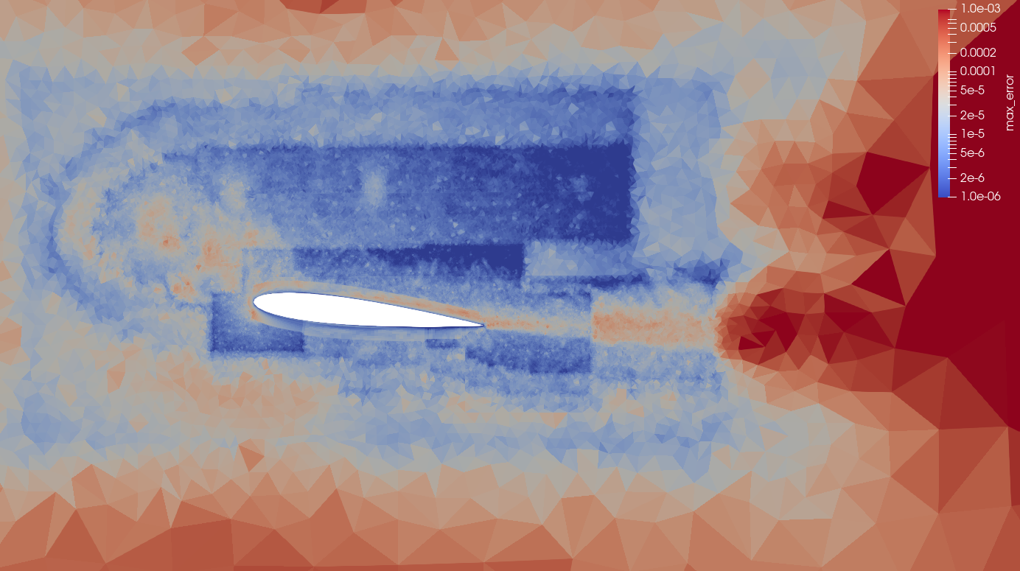
\includegraphics[width=1\textwidth]{figures/adapt_strat/FB_error_plot.png}
\caption{Mfa1\_nz50 error field}
\label{fig:FB_error_plot}
\end{subfigure}

\caption{Mesh and error-field for feature based strategy}
\end{figure}